\documentclass[11pt]{article}
\usepackage{fullpage,amsmath,amsfonts,mathpazo,microtype,nicefrac,graphicx}
\usepackage[font=footnotesize]{caption}
\usepackage{float}
%\usepackage{fancyhdr}
%\pagestyle{fancy}

% Set-up for hypertext references
\usepackage{hyperref,color,textcomp}
\definecolor{webgreen}{rgb}{0,.35,0}
\definecolor{webbrown}{rgb}{.6,0,0}
\definecolor{RoyalBlue}{rgb}{0,0,0.9}
\hypersetup{
  colorlinks=true, linktocpage=true, pdfstartpage=3, pdfstartview=FitV,
  breaklinks=true, pdfpagemode=UseNone, pageanchor=true, pdfpagemode=UseOutlines,
  plainpages=false, bookmarksnumbered, bookmarksopen=true, bookmarksopenlevel=1,
  hypertexnames=true, pdfhighlight=/O,
  urlcolor=webbrown, linkcolor=RoyalBlue, citecolor=webgreen,
  pdfauthor={Chris H. Rycroft},
  pdfsubject={Harvard AM205 (Fall 2017)},
  pdfkeywords={},
  pdfcreator={pdfLaTeX},
  pdfproducer={LaTeX with hyperref}
}
\hypersetup{pdftitle={notes}}

% Macro definitions
\newcommand{\N}{\mathbb{N}}
\newcommand{\Z}{\mathbb{Z}}
\newcommand{\Q}{\mathbb{Q}}
\newcommand{\R}{\mathbb{R}}
\newcommand{\B}{\mathbb{B}}
\newcommand{\p}{\partial}
\newcommand{\Trans}{\mathsf{T}}
\renewcommand{\vec}[1]{\mathbf{#1}}
\newcommand{\vx}{\vec{x}}
\newcommand{\vv}{\vec{v}}
\newcommand{\vb}{\vec{b}}
\newcommand{\sep}{\,|\,}
\newcommand{\suba}{\text{a}}
\newcommand{\subb}{\text{b}}
\newcommand{\subc}{\text{c}}
\newcommand{\subd}{\text{d}}

\DeclareMathOperator{\rank}{rank}

% Make LaTeX more willing to intermix figures and text
\renewcommand{\topfraction}{0.9}
\renewcommand{\bottomfraction}{0.8}
\renewcommand{\textfraction}{0.2}
\renewcommand{\floatpagefraction}{0.7}
\renewcommand{\dblfloatpagefraction}{0.7}

\title{Simplified Hydrostatic Carbon Burning in White Dwarf Interiors}
\author{Notes on the paper by Mehul Smriti Raje}

\begin{document}
\maketitle{}

\section{Problem Definition}
This project aims to develop a library to model and solve the set of nuclear reactions that occur in white dwarf interiors approaching ignition in SNeIa.

\section{Terms}
	\begin{itemize}
		\item $\lambda$ is the thermally averaged cross-section or rate of occurrence per particle per unit time - seems like fixed values.
		\item \textbf{Type Ia supernovae (SNeIa)} - thermonuclear explosion of white dwarf stars
		\item \textbf{White dwarf (WD) stars} - Stars composed of electron-degenerate matter; said to be the final stage of some stars.
		\item \textbf{CO WD} - Carbon Oxygen White Dwarf, i.e. White Dwarfs composed of carbon and Oxygen
	\end{itemize}

\section{Features of Proposed System}
	\begin{itemize}
		\item System takes in temperature and density values; initial C/O ratio given by nuclide mass fractions $X(^{12}C) = 0.3$ and $X(^{16}O) = 0.7$ but reasonable variations allowed.
		\item Find values of $\lambda$ 
		\item Find rates of different reactions at equilibrium
		\item Equilibrium mol fractions of trace nuclei can be calculated directly using Eq (13) in paper.
		\item Time scales can be calculated using equilibrium values. Alternatively, reverse calculation/missing values can be found using timescale information from given Table 1.
		\item System of equations can be solved to determine when equilibrium occurs, produce decay graphs.
		\item All values can be found in terms of the $^{12}C$ mol fractions.
	\end{itemize}	
	
	Stretch goals:	
	\begin{itemize}
		\item Find different behaviour for different concentration - is similar for reasonable changes to proposed ratio, but we might have to read more literature to do this.
	\end{itemize}

\section{Equations}
The graph describing consumption of 6 $^{12}C$ to produce four nuclei: 23Ne, 20Ne, 16O, and 13C and two $e^-$-captures is given by
	\begin{figure}[h]
		\centering
		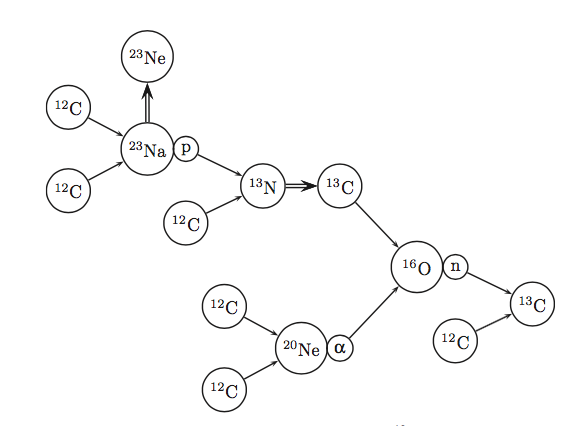
\includegraphics{resources/graph}
		\caption{Decomposition of $^{12}C$ nuclei}
	\end{figure}
	
	Some features of the system are
	\begin{itemize}
		\item Proton leaks: At low density ($<1.7$g cm$^{-3}$), $\beta$ decay time scale is shorter than $e^-$ capture, while for density ($>1.7$g cm$^{-3}$), $^{23}$Na $e^{-}$ capture time scale is shorter 
	\end{itemize}
	 
	
	The set of reactions occuring in the system can be written as
	\begin{align}
		&^{23}Na(p, \alpha)^{20}Ne, Q = 2.38 MeV\\
		&^{23}Na(p, \gamma)^{24}Mg, Q = 11.69 MeV\\
		&^{23}Ne(p, n)^{23}Na, Q = 3.59 MeV\\
		&^{20}Ne(n, \gamma)^{21}Ne, Q = 6.76 MeV\\
		&^{23}Na(n, \gamma)^{24}Na, Q = 6.96 MeV\\
		&^{12}C(\alpha, \gamma)^{16}O, Q = 7.16 MeV\\
		&^{16}O(\alpha, \gamma)^{20}Ne, Q = 2.84 MeV\\	
		&^{21}Ne(n, \gamma)^{22}Ne, Q = 10.36 MeV\\
	\end{align}
	\begin{align}
		&^{13}C(p, \gamma)^{14}N, Q = 7.55 MeV\\
		&^{21}Ne(p, \gamma)^{22}Na, Q = 6.74 MeV\\
		&^{20}Ne(\alpha, \gamma)^{24}Mg, Q = 9.32 MeV\\
		&^{23}Ne(\alpha, n)^{26}Mg, Q = 5.41 MeV\\
		&^{23}Na(\alpha, p)^{26}Mg, Q = 1.82 MeV\\
		&^{21}Ne(\alpha, n)^{26}Mg, Q = 4.84 MeV	
	\end{align} \\
	
	The set of differential equations arising from this set of reactions is given by
	\begin{figure}[H]
		\centering
		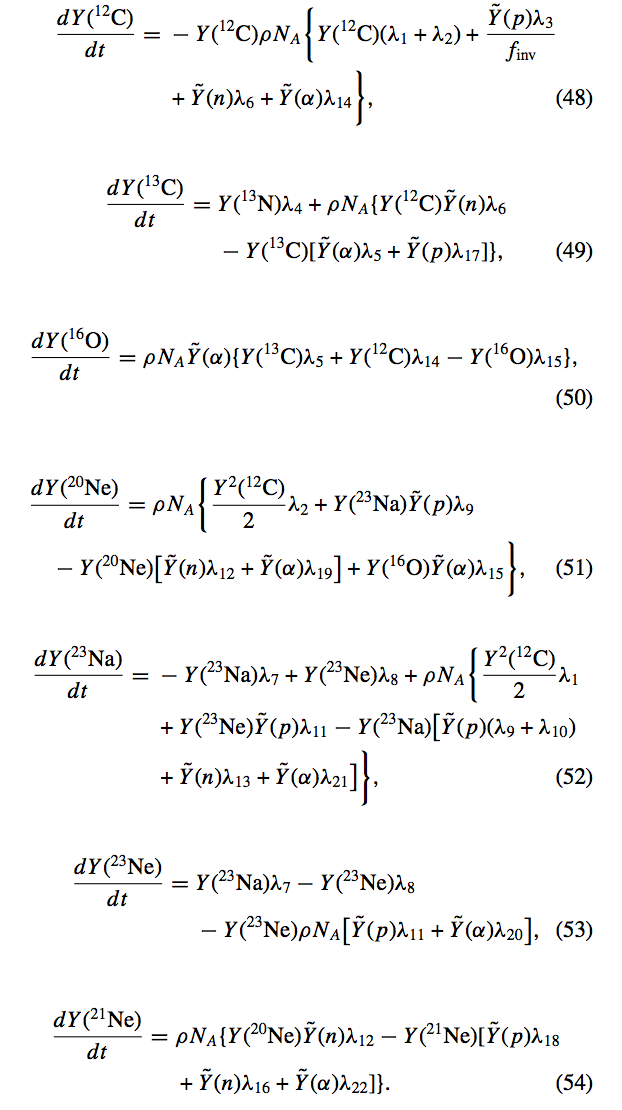
\includegraphics{resources/differential}
		\caption{Set of differential equations describing decomposition of $^{12}C$}
	\end{figure}	
	%\begin{align}
	%	& \frac{dY(^{12}C)}{dt}
	%\end{align}

\section{General Notes}
	\begin{enumerate}
		\item Degeneration of SNeIa progenitors
			\begin{itemize}
				\item Single Degenerate Scenario: CO WD accretes mass from a slightly evolved main-sequence companion (CO WD + MS), a more evolved red giant star (CO WD + RG), or a helium star (CO WD + He).
				\item Double Degenerate Scenario: CO WD forms as a result of the merger of two degenerate stars with a combined mass above the Chandrasekhar limit
			\end{itemize}
		\item Phases of evolution in the pre-explosion phase
		
			Conditions of system: High densities ($>10^7$ g cm$^{-3}$), high temperatures ($>108$ K),  environment rich in $^{12}C$ and $^{16}O$ nuclei and relatively devoid of free protons, $\alpha$-particles or neutrons. 
			\begin{itemize}
				\item Cooling phase 
					\begin{itemize}
						\item cooling to constant density after birth
					\end{itemize}						
				\item Accretion phase 
					\begin{itemize}
						\item shrinkage of star to maintain hydrostatic equilibrium
						\item adiabetic compression of core
						\item 
					\end{itemize}									
				\item Simmering phase 
					\begin{itemize}
						\item Compression at centre leads to burning of C and energy generation
						\item Energy convectively transferred from core and can engulf whole star
						\item Convective Urca process, i.e. $e^-$ and $\beta-$ decays at high density
					\end{itemize}					
				\item Thermonuclear flash
					\begin{itemize}
						\item Energy gain $>$ Energy Loss 
						\item Central temperature of star increases at constant density
					\end{itemize}					
				\item Thermonuclear runway
					\begin{itemize}
						\item Ignition spots give rise to nuclear flame if temperature is high enough
						\item Deflagration wave converts to detonation wave sometimes
						\item Waves contribute to the kinetic energy of ejecta, radioactive matter forming light curve of supernova
						\item Much shorter phase
					\end{itemize}					
			\end{itemize}
		\item The ejecta in SNeIa explosion are determined by the pre-supernova evolution of WDs.
		\item C burning pollutes the WD core with ashes.
		\item N1 traces the decay of major elements to generate $^{13}C$ from $^{12}C$.
		\item N2 includes the effects of leak reactions that occur at different densities due to different rates of production of reacting species. This produces properties of full network at 5\% level, i.e. its time evolution reflects the time evolution of the full network.
	\end{enumerate}

\end{document}
